\problem{}
We are given an $n \times m$ array of cells. Denote the cell in the $r$'th row and the $c$'th column as $(r,c)$, where $1 \leq r \leq n$ and $1 \leq c \leq m$. A robot is at cell $(1, 1)$ and wants to reach cell $(n, m)$. From cell $(x, y)$, the robot can only move to $(x,y+1)$ or $(x+1,y)$. In addition, some cells contain impassable obstacles and the robot cannot move to these cells. Your goal is to put additional obstacles in the minimum number of cells (other than cell $(n, m)$) such that the robot cannot reach $(n, m)$.  Find an algorithm based on max flow.  

\solution{}
\begin{figure}[htbp]
    \centering
    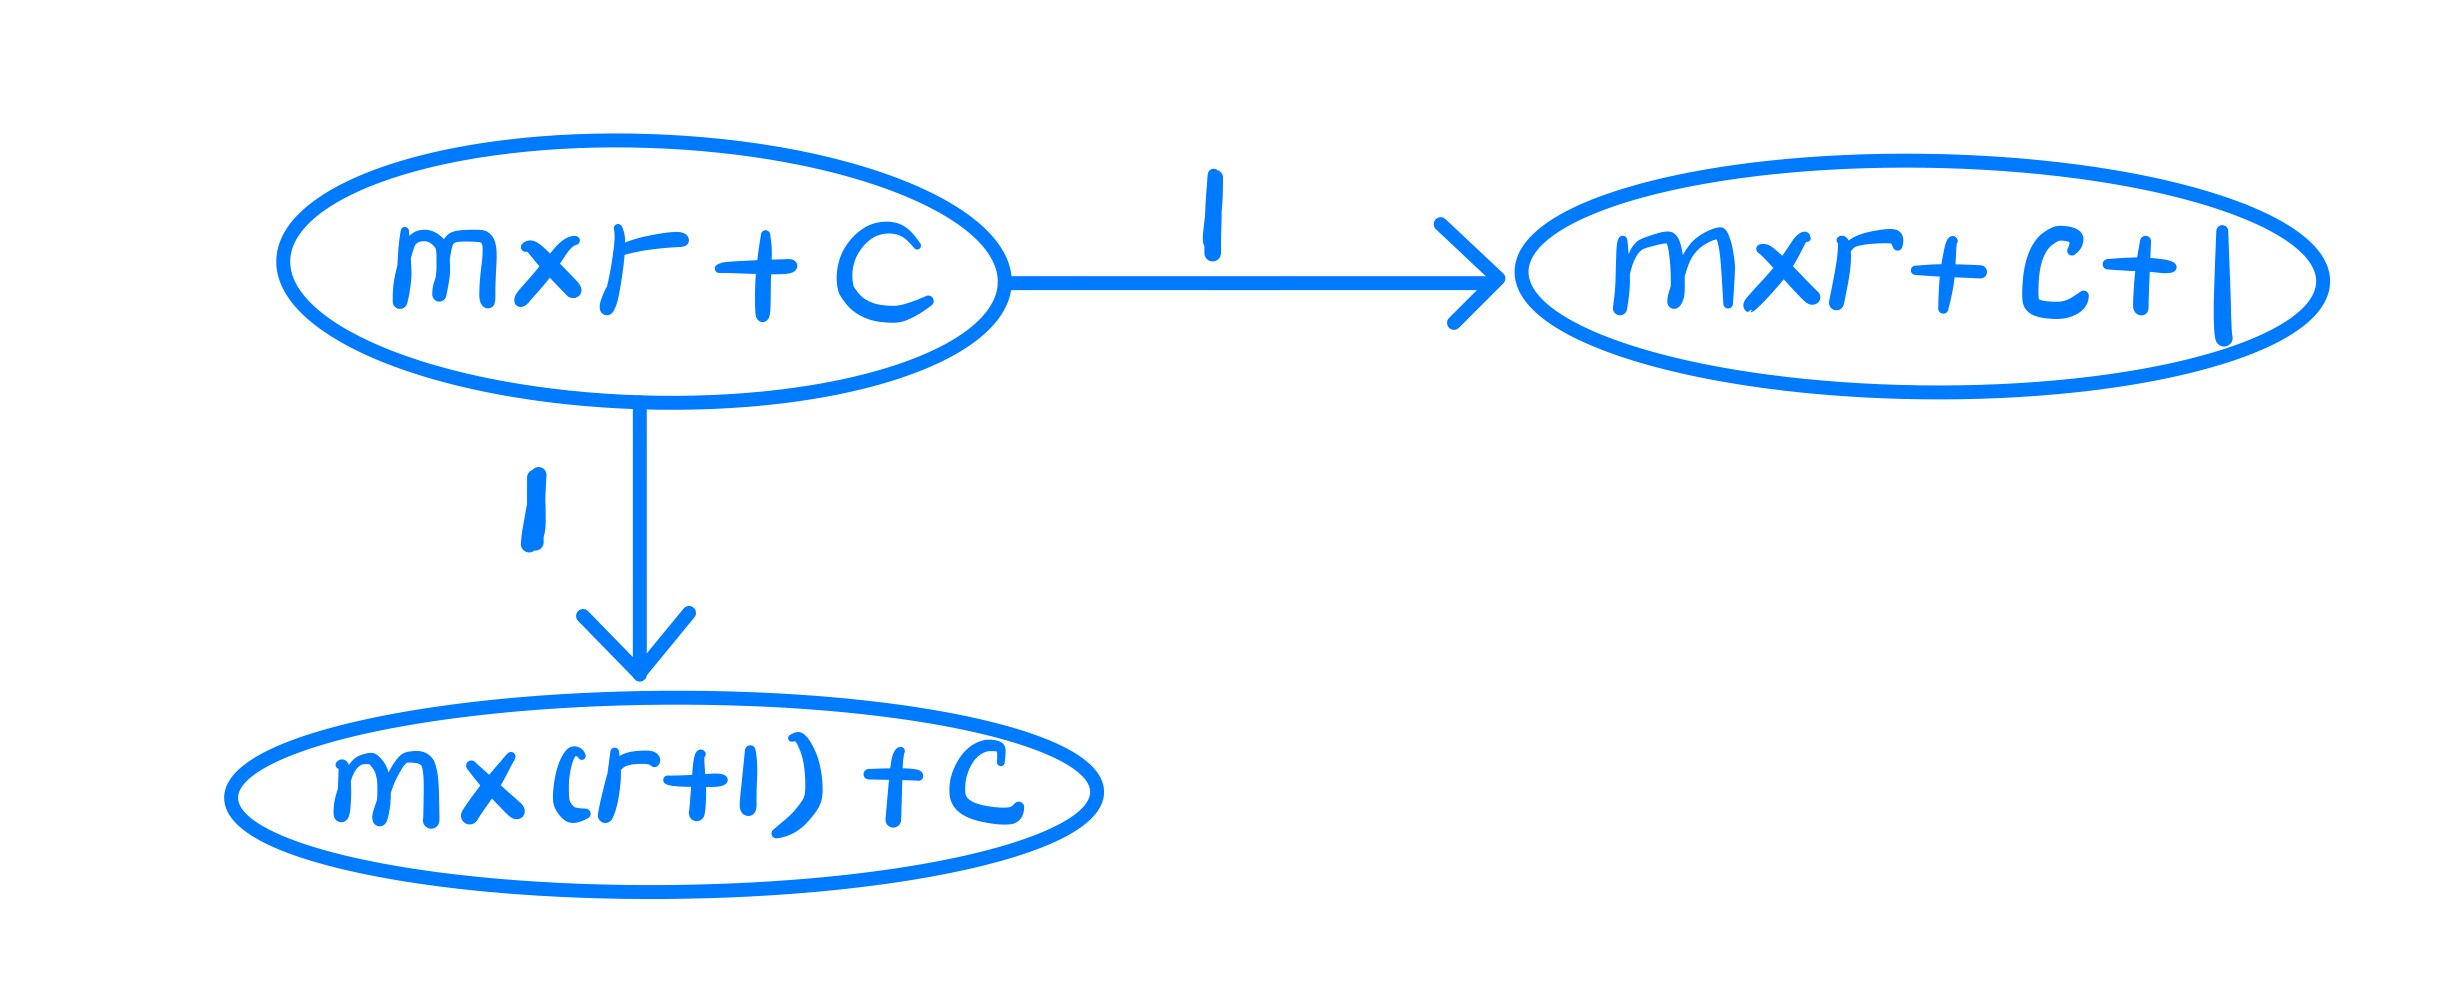
\includegraphics[width=\linewidth]{../fig/p2.png}
    \caption{Way to contrust the graph}
    \label{fig:p2}
\end{figure}

We can construct the graph as the Figure \ref{fig:p2} shows.

The details are as follows:\\
For a cell whose location is $(r,c)$, we can give it a number $m*r+c$ as the node's number.\\
Since from cell $(r,c)$, we can reach $(r+1,c)$ or $(r,c+1)$ is there is no obstacles.\\
So we can construct the graph:\\
If there is no obstacle on $(r,c)$ and $(r+1,c)$, then we set up an edge from node $m*r+c$ to node $m*(r+1)+c$, and the capacity is $1$.\\
If there is no obstacle on $(r,c)$ and $(r,c+1)$, then we set up an edge from node $m*r+c$ to node $m*r+c+1$, and the capacity is $1$.\\

After constructed the map, since we start from $(1,1)$ to $(n,m)$, so we can regard the node representing $(1,1)$ to be the source node $s$, and the node representing $(n,m)$ to be the sink node $t$.\\
Since we want to get the minimum number of obstacles to put, we can actually getting the minimum cut of the constructed graph.\\
For an edge $(u,v)$, if it is in the minimum cut and $v\neq t$, then we can put an obstacle to the grid representing to the node $v$.\\
If $(u,v)$ is in the minimum cut and $v = t$, then we can put an obstacle to the grid representing to the node $u$.\\
Then we can get the minimum cut to get the places to put the obstacles.\\

Since what we have learned that the minimum $s-t$ cut is the same as the maximum flow.\\
So we can use the Ford-Fulkerson algorithm to find the maximum flow of the constructed graph. \\

So the minimum number of obstacles we need to set is the maximum flow on the constructed graph. \\
And the methods to set up obstacles are mentioned above.\\
The time complexity is $O(n^2m^2)$.\\
Since there are total $nm$ nodes, and there will have atmost $2$ edges come out from each node. And all the edge's capacity is $1$.\\

\newpage